\documentclass[12pt]{article}
\usepackage[utf8]{inputenc}
\usepackage{graphicx}
\usepackage{titling}
\usepackage{datetime}
\usepackage{enumitem}
\usepackage{xcolor}
\usepackage{listings}
\usepackage{multirow}

% Título de la tarea
\title{\vspace{1cm}Proyecto Final de Bases de Datos}
\date{} % Deja la fecha en blanco

% Ajustar márgenes para la portada
\usepackage[left=3cm,right=3cm,top=3cm,bottom=3cm]{geometry}

% Comando para agregar los escudos
\newcommand{\doubleshield}[2]{%
    \begin{minipage}[t]{0.48\textwidth}
        \centering
        \includegraphics[width=0.5\linewidth]{#1}
        \par\vspace{1ex}
        %Escudo #1
    \end{minipage}\hfill%
    \begin{minipage}[t]{0.48\textwidth}
        \centering
        \includegraphics[width=0.5\linewidth]{#2}
        \par\vspace{1ex}
        %Escudo #2
    \end{minipage}%
}

\begin{document}

\lstset{
    language=SQL,                   % Lenguaje de programación
    basicstyle=\ttfamily,              % Fuente y estilo básico
    keywordstyle=\color{red},         % Estilo de las palabras clave
    commentstyle=\color{green},        % Estilo de los comentarios
    numbers=left,                      % Números de línea a la izquierda
    numberstyle=\tiny\color{gray},     % Estilo de los números de línea
    frame=single,                      % Borde alrededor del código
    breaklines=true,                   % Romper líneas largas
    postbreak=\mbox{\textcolor{red}{$\hookrightarrow$}\space}, % Flecha de ruptura de línea
    showstringspaces=false             % No mostrar espacios en cadenas
}


\pagecolor{black}
\color{white}

\begin{titlepage}
    \begin{center}
        \vspace*{2cm}
        
        % Agrega los escudos aquí
        \doubleshield{UNAM.png}{EFC.png}
        
        \vspace{2cm}
        
        \Huge{\thetitle}
        
        \vspace{4cm}
        
        \Large{Tarea presentada por:}
        
        \vspace{0.5cm}
        
        \Large{Edgar Montiel Ledesma 317317794 \\ Carlos Daniel Cortes Jimenez 420004846}
        
        \vfill
        
        Facultad de Ciencias \\
        Universidad Nacional Autónoma de Méixco \\
        Fecha de Entrega: 11 de Diciembre de 2023 % Cambia la fecha de entrega        
    \end{center}
\end{titlepage}
    
    \section*{Base de Datos: Sistema de Administración de Tienda en Línea}

    \subsection*{1. Lista de Requerimientos}
    % Lista de requerimientos aquí
        \begin{itemize}
            \item[1.] Registro de Clientes:
                \begin{itemize}
                    \item La base de datos debe permitir el registro de nuevos clientes, incluyendo su nombre, dirección y número de teléfono.
                \end{itemize}
            \item[2.] Registro de Autos:
                \begin{itemize}
                    \item La base de datos debe permitir el registro de nuevos autos, incluyendo información como modelo, marca, año de fabricación y precio.
                \end{itemize}
            \item[3.] Registro de Empleados:
                \begin{itemize}
                    \item La base de datos debe permitir el registro de empleados, especificando su nombre, dirección, número de teléfono y rol en la agencia (gerente, asesor, promotor, mecánico, electromecánico, etc.).
                \end{itemize}
            \item[4.] Registro de Servicios:
                \begin{itemize}
                    \item La base de datos debe permitir el registro de servicios ofrecidos por la agencia, incluyendo nombre del servicio, descripción y precio.
                \end{itemize}
            \item[5.] Registro de Mantenimientos:
                \begin{itemize}
                    \item La base de datos debe permitir el registro de mantenimientos realizados, especificando el auto involucrado, el cliente, el empleado a cargo, el servicio proporcionado y la fecha del mantenimiento.
                \end{itemize}
            \item[6.] Registro de Trabajos de Hojalatería y Pintura:
                \begin{itemize}
                    \item La base de datos debe permitir el registro de trabajos de hojalatería y pintura, indicando el auto, el cliente, el empleado responsable, el servicio proporcionado y la fecha del trabajo.
                \end{itemize}
            \item[7.] Registro de Seguros para Autos:
                \begin{itemize}
                    \item La base de datos debe permitir el registro de seguros para autos, detallando el auto asegurado, el cliente, el tipo de seguro, la cobertura y el precio del seguro.
                \end{itemize}
            \item[8.] Relaciones entre Entidades:
                \begin{itemize}
                    \item La base de datos debe establecer y mantener relaciones adecuadas entre las entidades, como la asociación de autos con clientes, empleados con mantenimientos y servicios con mantenimientos.
                \end{itemize}
            \item[9.] Consulta de Información:
                \begin{itemize}
                    \item Debe ser posible realizar consultas para obtener información detallada, como el historial de mantenimientos de un auto, los clientes asociados a un empleado.
                \end{itemize}
            \item[10.] Integridad Referencial:
                \begin{itemize}
                    \item La base de datos debe garantizar la integridad referencial, asegurando que las claves foráneas estén correctamente vinculadas a las claves primarias correspondientes.
                \end{itemize}
            \item[11.] Manejo de Precios en Decimal:
                \begin{itemize}
                    \item Los precios deben manejarse con precisión decimal, considerando los campos que almacenan valores monetarios.
                \end{itemize}
            \item[12.] Registro de Fechas:
                \begin{itemize}
                    \item La base de datos debe almacenar fechas de manera precisa para rastrear la temporalidad de eventos como mantenimientos, trabajos de hojalatería y pintura.
                \end{itemize}
        \end{itemize}

    \subsection*{2. Modelo Conceptual (Notación de Peter Chen)}
    \begin{figure}[h]
        \centering
        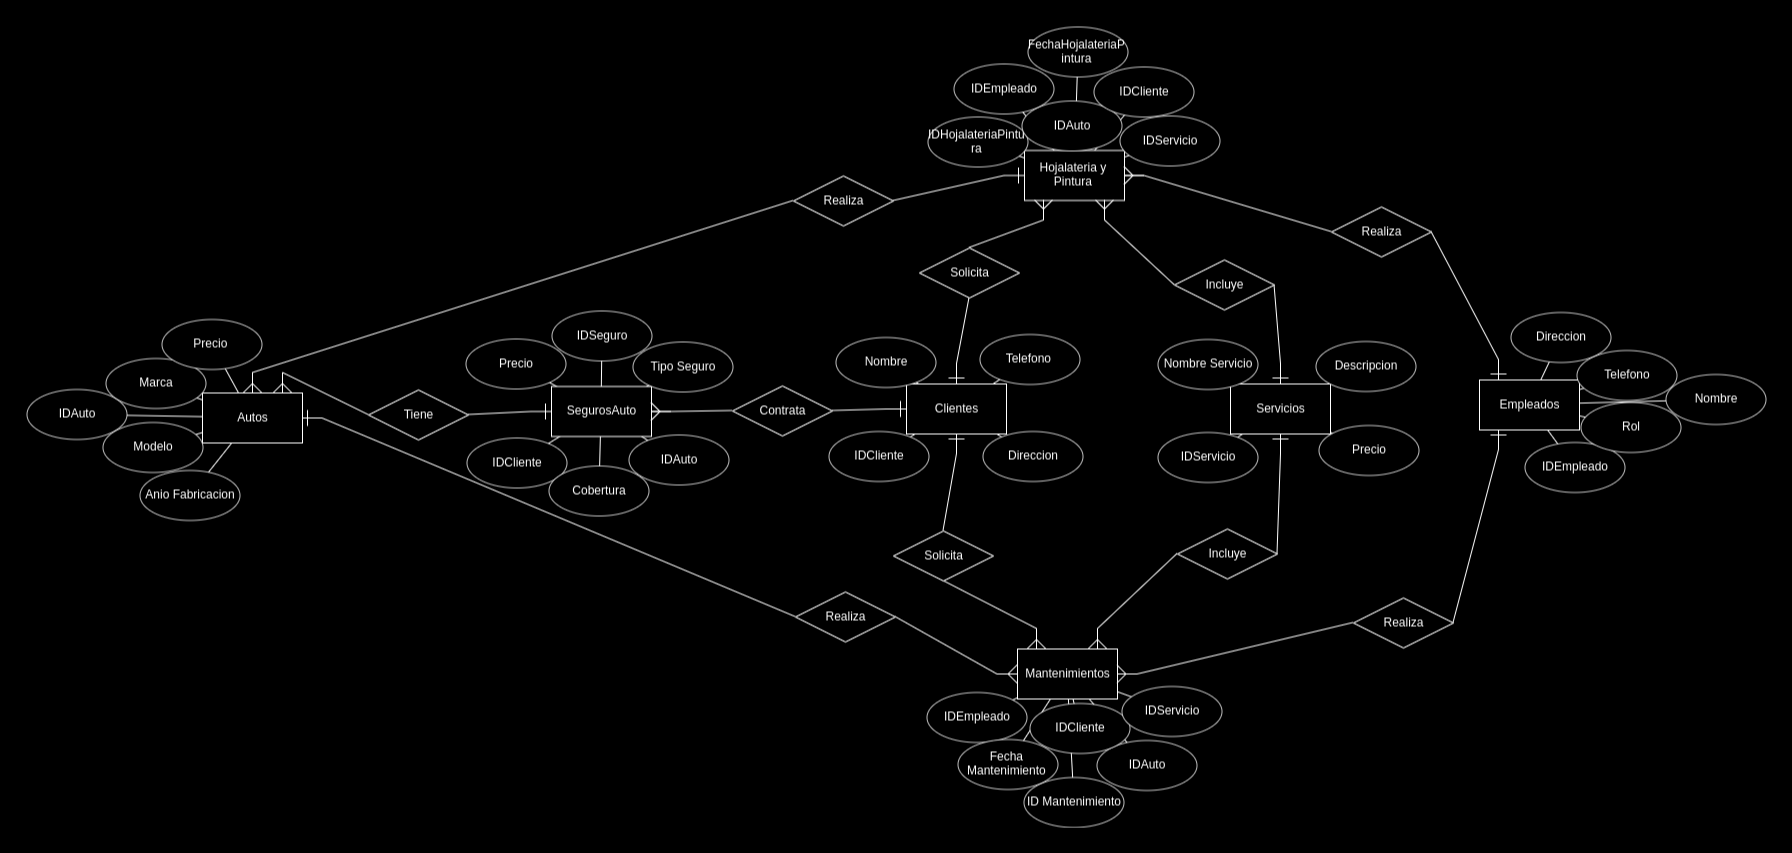
\includegraphics[width=0.9\textwidth]{EAuto.png}
        \caption{Modelo Conceptual}
        \label{fig:modelo-conceptual}
    \end{figure}

    \subsection*{3. Modelo Relacional}
    \begin{figure}[h]
        \centering
        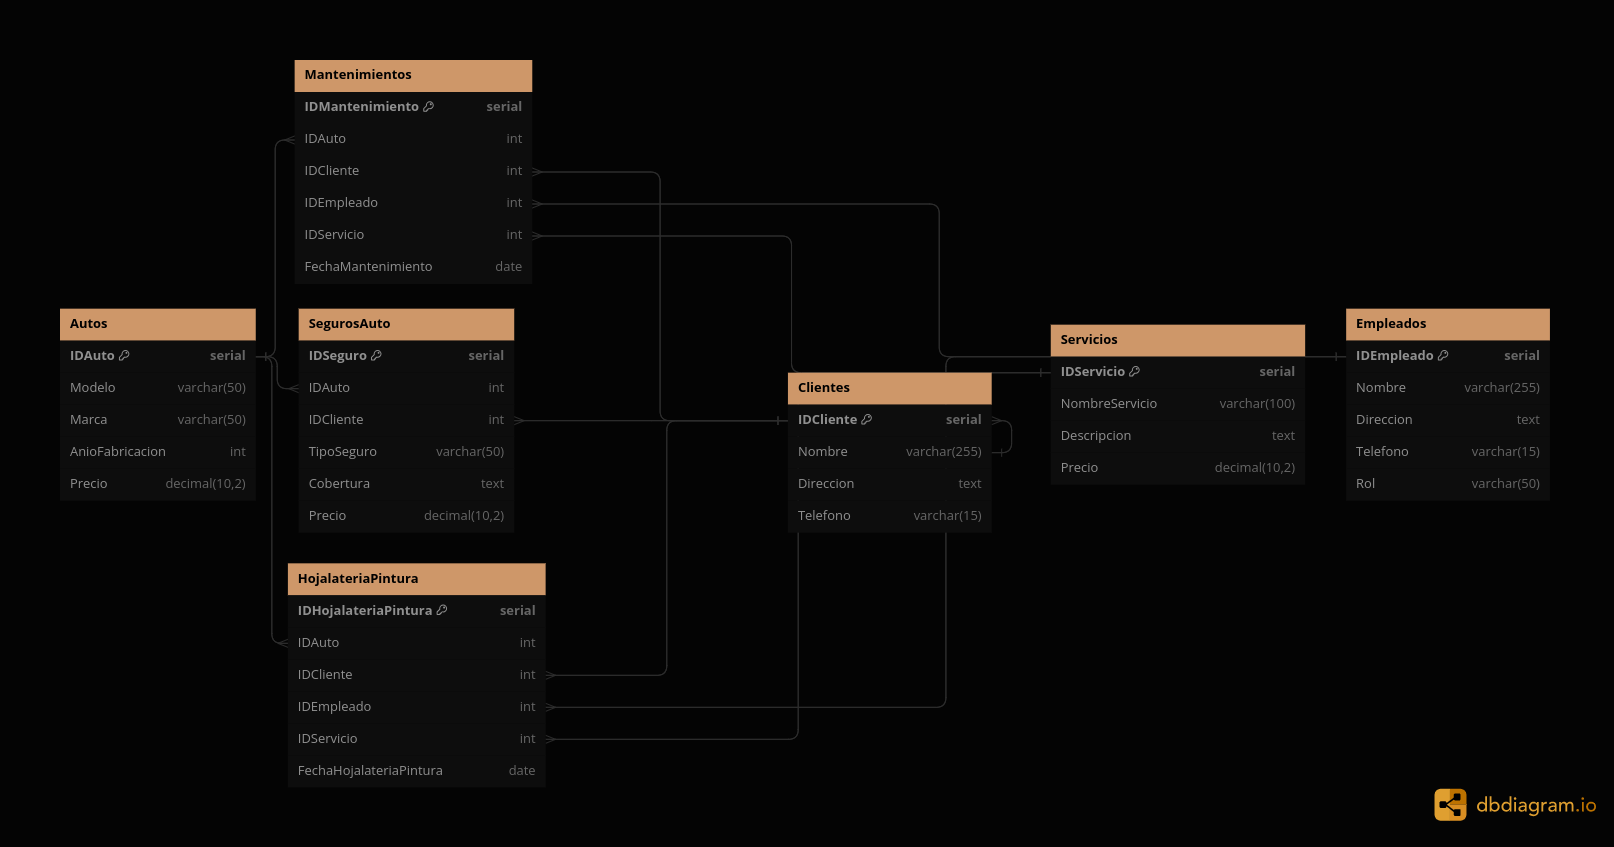
\includegraphics[width=1.0\textwidth]{ERAuto.png}
        \caption{Modelo Conceptual}
        \label{fig:modelo-conceptual}
    \end{figure}

    \subsection*{4. Script Completo para Crear la Base de Datos}
    \begin{lstlisting}[language=SQL]
-- Creacion de Tablas
CREATE TABLE "Clientes" (
  "IDCliente" serial PRIMARY KEY,
  "Nombre" varchar(255) NOT NULL,
  "Direccion" text NOT NULL,
  "Telefono" varchar(15) NOT NULL CHECK(length("Telefono") > 0)
);

CREATE TABLE "Autos" (
  "IDAuto" serial PRIMARY KEY,
  "Modelo" varchar(50) NOT NULL,
  "Marca" varchar(50) NOT NULL,
  "AnioFabricacion" int NOT NULL CHECK("AnioFabricacion" > 0),
  "Precio" decimal(10,2) NOT NULL CHECK("Precio" >= 0.0)
);

CREATE TABLE "Empleados" (
  "IDEmpleado" serial PRIMARY KEY,
  "Nombre" varchar(255) NOT NULL,
  "Direccion" text NOT NULL,
  "Telefono" varchar(15) NOT NULL CHECK(length("Telefono") > 0),
  "Rol" varchar(50) NOT NULL
);

CREATE TABLE "Servicios" (
  "IDServicio" serial PRIMARY KEY,
  "NombreServicio" varchar(100) NOT NULL,
  "Descripcion" text NOT NULL,
  "Precio" decimal(10,2) NOT NULL CHECK("Precio" >= 0.0)
);

CREATE TABLE "Mantenimientos" (
  "IDMantenimiento" serial PRIMARY KEY,
  "IDAuto" int NOT NULL,
  "IDCliente" int NOT NULL,
  "IDEmpleado" int NOT NULL,
  "IDServicio" int NOT NULL,
  "FechaMantenimiento" date NOT NULL,
  FOREIGN KEY ("IDAuto") REFERENCES "Autos"("IDAuto") ON DELETE CASCADE ON UPDATE CASCADE,
  FOREIGN KEY ("IDCliente") REFERENCES "Clientes"("IDCliente") ON DELETE CASCADE ON UPDATE CASCADE,
  FOREIGN KEY ("IDEmpleado") REFERENCES "Empleados"("IDEmpleado") ON DELETE CASCADE ON UPDATE CASCADE,
  FOREIGN KEY ("IDServicio") REFERENCES "Servicios"("IDServicio") ON DELETE CASCADE ON UPDATE CASCADE
);

CREATE TABLE "HojalateriaPintura" (
  "IDHojalateriaPintura" serial PRIMARY KEY,
  "IDAuto" int NOT NULL,
  "IDCliente" int NOT NULL,
  "IDEmpleado" int NOT NULL,
  "IDServicio" int NOT NULL,
  "FechaHojalateriaPintura" date NOT NULL,
  FOREIGN KEY ("IDAuto") REFERENCES "Autos"("IDAuto") ON DELETE CASCADE ON UPDATE CASCADE,
  FOREIGN KEY ("IDCliente") REFERENCES "Clientes"("IDCliente") ON DELETE CASCADE ON UPDATE CASCADE,
  FOREIGN KEY ("IDEmpleado") REFERENCES "Empleados"("IDEmpleado") ON DELETE CASCADE ON UPDATE CASCADE,
  FOREIGN KEY ("IDServicio") REFERENCES "Servicios"("IDServicio") ON DELETE CASCADE ON UPDATE CASCADE
);

CREATE TABLE "SegurosAuto" (
  "IDSeguro" serial PRIMARY KEY,
  "IDAuto" int NOT NULL,
  "IDCliente" int NOT NULL,
  "TipoSeguro" varchar(50) NOT NULL,
  "Cobertura" text NOT NULL,
  "Precio" decimal(10,2) NOT NULL CHECK("Precio" >= 0.0),
  FOREIGN KEY ("IDAuto") REFERENCES "Autos"("IDAuto") ON DELETE CASCADE ON UPDATE CASCADE,
  FOREIGN KEY ("IDCliente") REFERENCES "Clientes"("IDCliente") ON DELETE CASCADE ON UPDATE CASCADE
);
    \end{lstlisting}

    \subsection*{5. Script de Inserción de Datos (para 100 registros)}
    La inserción de datos, se encuentra en el archivo Automotriz-insert.sql, no se colocaron los 100 registros para la tabla Servicios, Mantenimientos, HojalateriaPintura y SegurosAuto ya que es una agencia de autos con que atiende una solo marca, ademas de que no se puede garantizar que los 100 autos o 100 clientes soliciten servicios o aseguren el automovil con la agencia.
    

    \subsection*{6. Evidencia de Restricciones de Integridad Referencial}
    \begin{itemize}
        \item[1.] En la tabla Mantenimientos:
        \begin{itemize}
            \item FOREIGN KEY ("IDAuto") REFERENCES "Autos"("IDAuto") ON DELETE CASCADE ON UPDATE CASCADE: Esto indica que el campo IDAuto en la tabla Mantenimientos está relacionado con el campo IDAuto en la tabla Autos. Si un registro en la tabla Autos se elimina o se actualiza, los registros correspondientes en la tabla Mantenimientos también se eliminarán o se actualizarán en cascada.
            \item FOREIGN KEY ("IDCliente") REFERENCES "Clientes"("IDCliente") ON DELETE CASCADE ON UPDATE CASCADE: Similar al caso anterior, la relación entre IDCliente en Mantenimientos y IDCliente en Clientes.
            \item FOREIGN KEY ("IDEmpleado") REFERENCES "Empleados"("IDEmpleado") ON DELETE CASCADE ON UPDATE CASCADE: Igual que los anteriores, asegura la integridad referencial entre IDEmpleado en Mantenimientos y IDEmpleado  en Empleados.
            \item FOREIGN KEY ("IDServicio") REFERENCES "Servicios"("IDServicio") ON DELETE CASCADE ON UPDATE CASCADE:  Similar al caso anterior, la relación entre IDServicio en Mantenimientos y IDServicio en Servicios.
        \end{itemize}
        \item[2.] En la tabla HojalateriaPintura:
        \begin{itemize}
            \item Se establecen relaciones similares a las de Mantenimientos con las tablas Autos, Clientes, Empleados y Servicios.
        \end{itemize}
        \item[3.] En la tabla SegurosAuto:
        \begin{itemize}
            \item FOREIGN KEY ("IDAuto") REFERENCES "Autos"("IDAuto") ON DELETE CASCADE ON UPDATE CASCADE: Asegura la integridad referencial entre IDAuto en SegurosAuto y IDAuto en Autos.
            \item FOREIGN KEY ("IDCliente") REFERENCES "Clientes"("IDCliente") ON DELETE CASCADE ON UPDATE CASCADE: Similar al caso anterior, la relación entre IDCliente en SegurosAuto y IDCliente en Clientes.
        \end{itemize}
    \end{itemize}
    Estas restricciones de integridad referencial garantizan que, en caso de eliminar o actualizar un registro en las tablas referenciadas, las acciones correspondientes se llevarán a cabo en las tablas que contienen las claves foráneas, manteniendo así la coherencia en la base de datos.\\
    Como se muestra en el siguente ejemplo de la elimincion y atualizacion en cascada.\\

        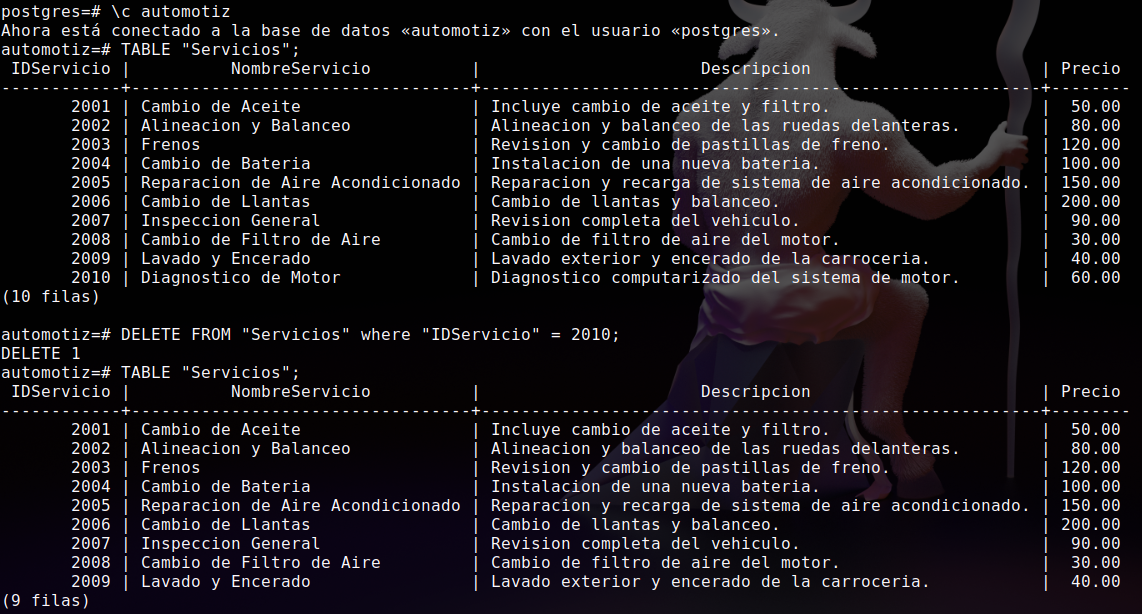
\includegraphics[width=1.0\textwidth]{Prueba1.png}
        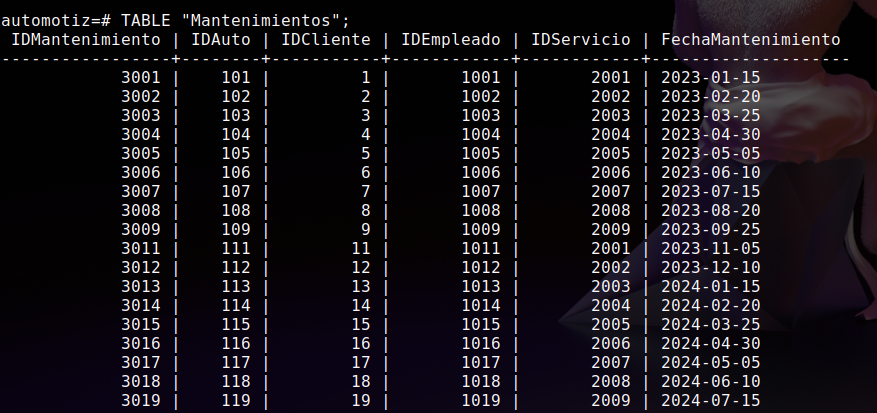
\includegraphics[width=1.0\textwidth]{Prueba2.png}

    \subsection*{7. Evidencia de Restricciones CHECK}
    \begin{itemize}
        \item[1.] Tabla involucrada en la restricción:
            \item Autos.
        \item[2.] Columnas involucradas en la restricción:
            \item AnioFabricacion.
            \item Precio.
        \item[3.] Definición de la restricción CHECK:
            \item En la creación de la tabla Autos, agregar una restricción CHECK a las columnas mencionadas:
        \begin{lstlisting}
CREATE TABLE "Autos" (
  "IDAuto" serial PRIMARY KEY,
  "Modelo" varchar(50),
  "Marca" varchar(50),
  "AnioFabricacion" int CHECK (AnioFabricacion > 1900),
  "Precio" decimal(10,2) CHECK (Precio >= 0)
);
        \end{lstlisting}
        \item[4.] Instrucción INSERT que viola la restricción:
        \begin{lstlisting}
INSERT INTO Autos ("Modelo", "Marca", "AnioFabricacion", "Precio") VALUES ('Sedan', 'Toyota', 1800, 25000.00);
        \end{lstlisting}
        \item[5.] Captura de pantalla con el resultado de la instrucción que muestra que la restricción está funcionando:
            \item Antes de aplicar INSERT:
            \center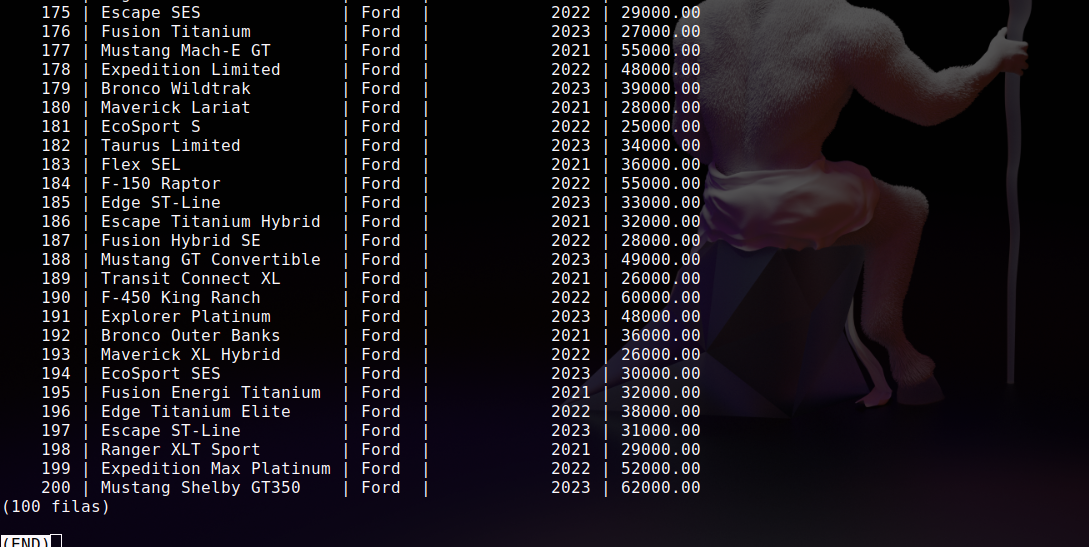
\includegraphics[width=1.0\textwidth]{A.png}
            \item Después de aplicar INSERT:
            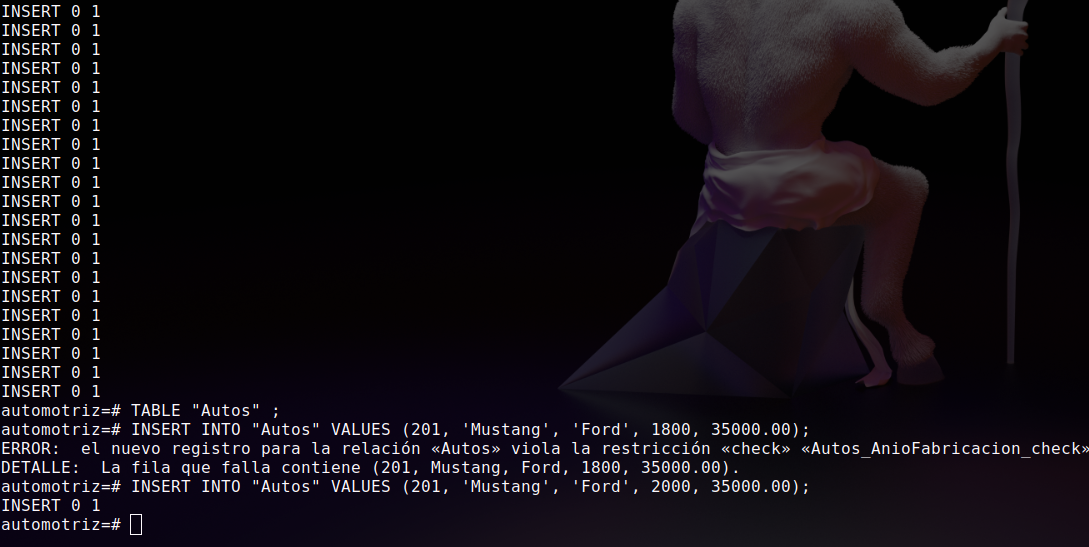
\includegraphics[width=1.0\textwidth]{B.png}
        \item[6.] Instrucción INSERT que cumple con la restricción:
        \begin{lstlisting}
INSERT INTO Autos ("Modelo", "Marca", "AnioFabricacion", "Precio") VALUES ('Sedan', 'Toyota', 2005, 25000.00);
        \end{lstlisting}
        \item[7.] Captura de pantalla con el resultado de la instrucción que muestra que la restricción está funcionando:
        \item Antes de aplicar INSERT:
        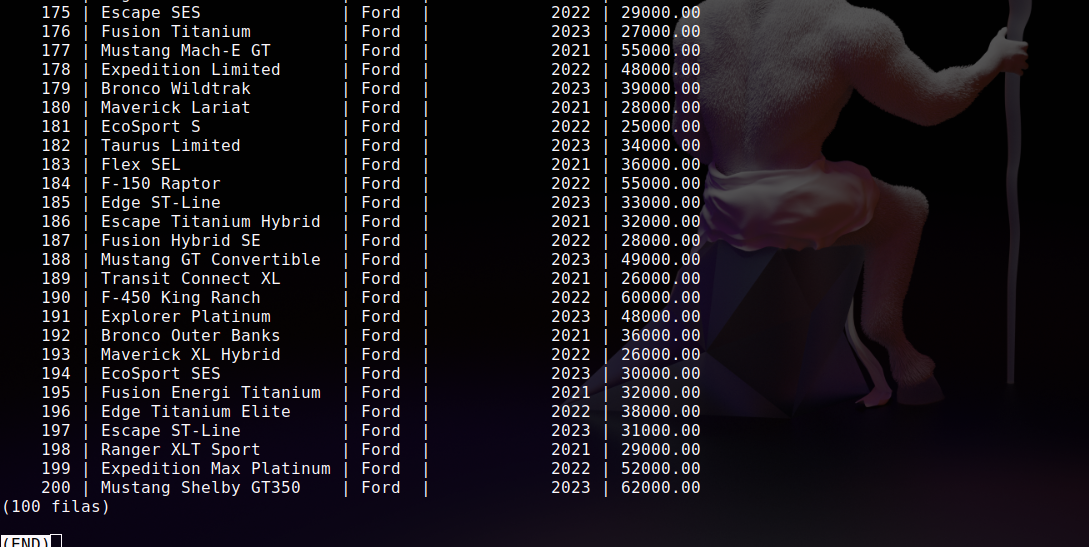
\includegraphics[width=1.0\textwidth]{A.png}
        \item Después de aplicar INSERT:
        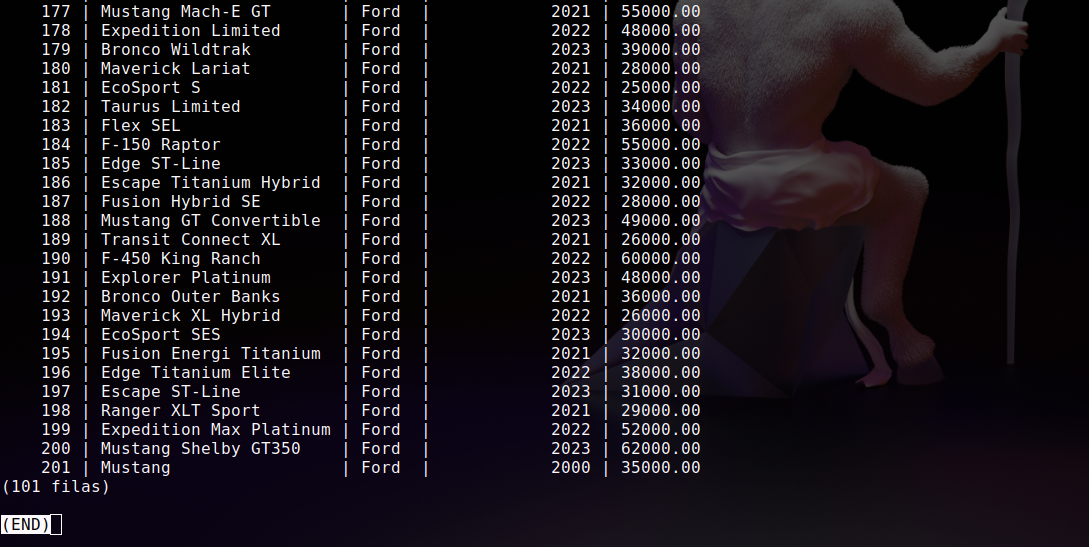
\includegraphics[width=1.0\textwidth]{C.png}
    \end{itemize}
    
    \subsection*{8. Evidencia de Dominios Personalizados}
    \begin{itemize}
        \item[1.] Dominio personalizado definido:
            \item Definimos un dominio personalizado llamado ModeloAutomovil que tiene una longitud máxima de 30 caracteres.
        \begin{lstlisting}
CREATE DOMAIN ModeloAutomovil AS varchar(30);
        \end{lstlisting}
        \item[2.] Uso del dominio personalizado en la creación de la tabla:
            \item Al crear la tabla Autos, utilizamos el dominio personalizado para la columna Modelo.
        \begin{lstlisting}
CREATE TABLE "Autos" (
  "IDAuto" serial PRIMARY KEY,
  "Modelo" ModeloAutomovil,
  "Marca" varchar(50),
  "AnioFabricacion" int,
  "Precio" decimal(10,2)
);
        \end{lstlisting}
        \item[3.] Instrucción INSERT que viola la restricción del dominio:
        \begin{lstlisting}
INSERT INTO Autos ("Modelo", "Marca", "AnioFabricacion", "Precio") VALUES ('EsteModeloEsMuyLargoYViolaraLaRestriccion', 'Toyota', 2005, 25000.00);
        \end{lstlisting}
        \item[4.] Captura de pantalla con el resultado de la instrucción que muestra que la restricción está funcionando:
        \item Antes de aplicar INSERT:
        \center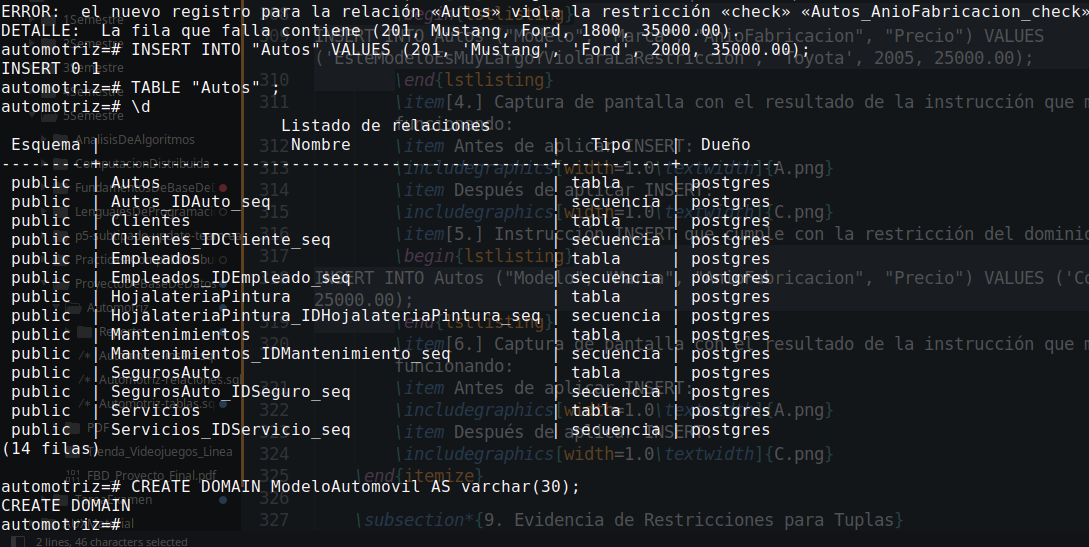
\includegraphics[width=1.0\textwidth]{D.png}
        \item Después de aplicar INSERT:
        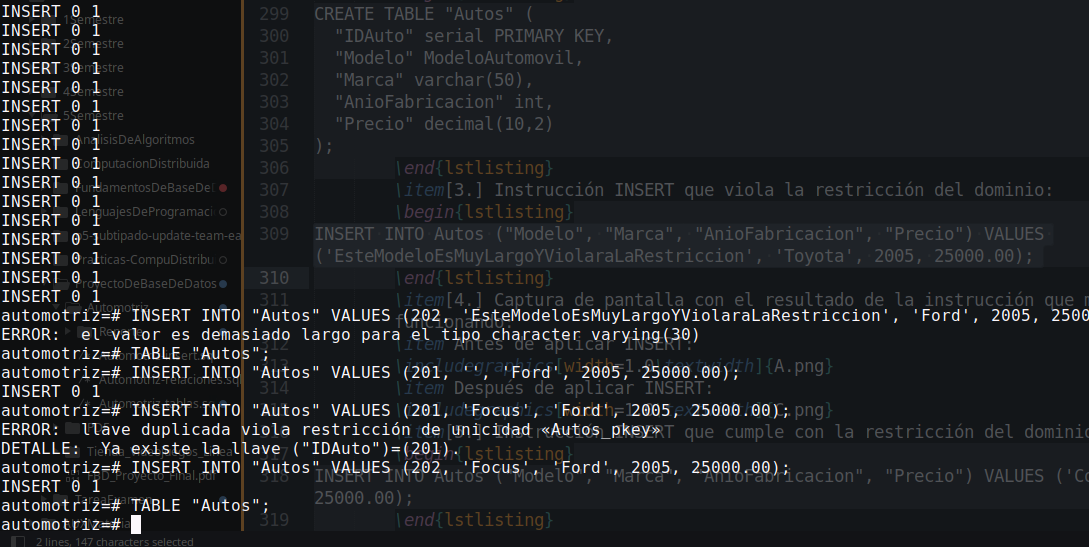
\includegraphics[width=1.0\textwidth]{E.png}
        \item[5.] Instrucción INSERT que cumple con la restricción del dominio:
        \begin{lstlisting}
INSERT INTO Autos ("Modelo", "Marca", "AnioFabricacion", "Precio") VALUES ('Corolla', 'Toyota', 2005, 25000.00);            
        \end{lstlisting}
        \item[6.] Captura de pantalla con el resultado de la instrucción que muestra que la restricción está funcionando:
        \item Antes de aplicar INSERT:
        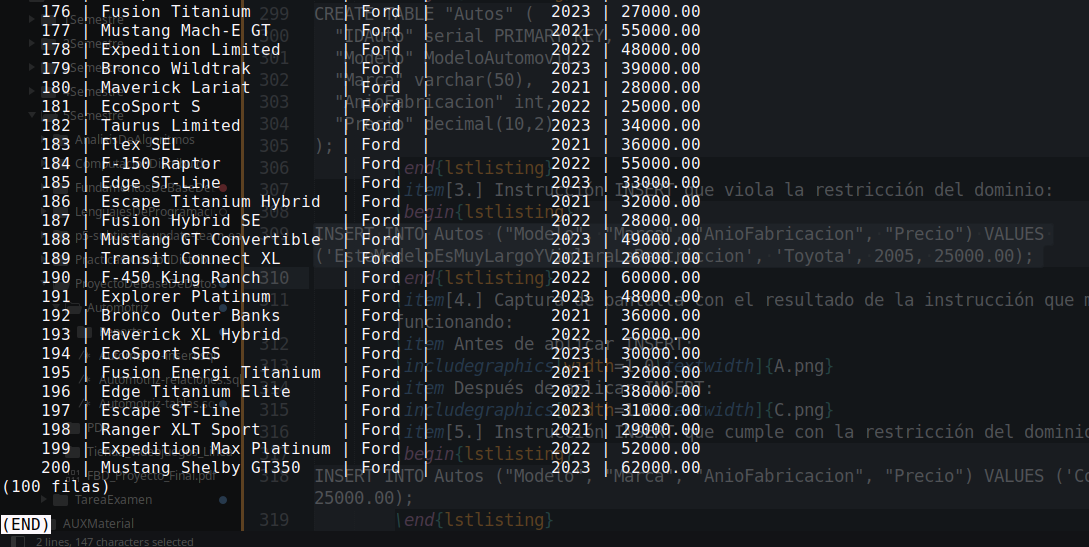
\includegraphics[width=1.0\textwidth]{F.png}
        \item Después de aplicar INSERT:
        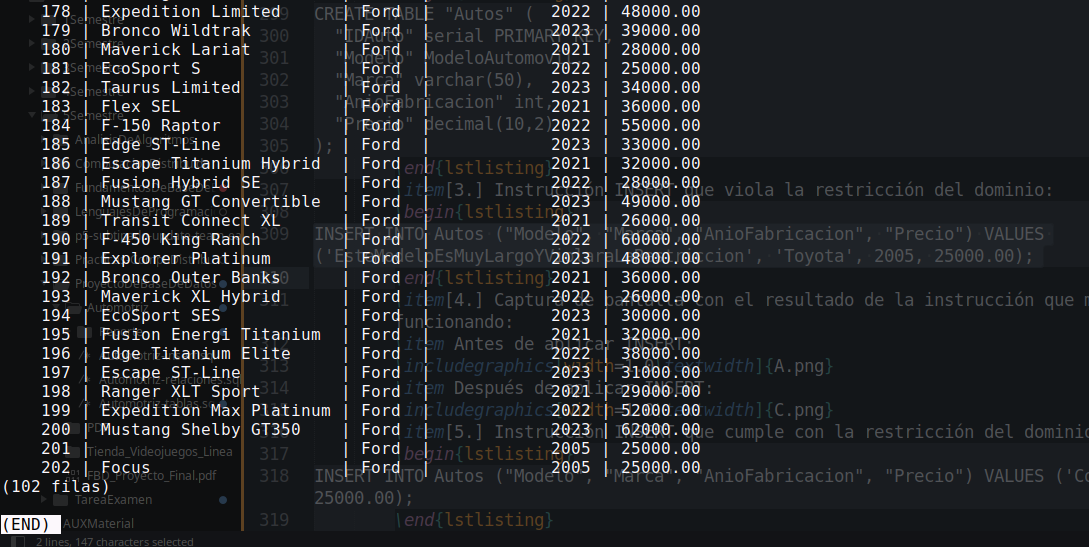
\includegraphics[width=1.0\textwidth]{G.png}
    \end{itemize}
    
    \subsection*{9. Evidencia de Restricciones para Tuplas}
    \begin{itemize}
        \item[1.] Restricción CHECK para tuplas definida en la creación de la tabla Mantenimientos:
        \item Agregamos una restricción CHECK para cada fila de la tabla Mantenimientos que asegure que la fecha de mantenimiento sea posterior al año de fabricación y que el servicio esté registrado en la tabla Servicios.
        \begin{lstlisting}
CREATE TABLE "Mantenimientos" (
  "IDMantenimiento" serial PRIMARY KEY,
  "IDAuto" int,
  "IDCliente" int,
  "IDEmpleado" int,
  "IDServicio" int,
  "FechaMantenimiento" date,
  CHECK ("FechaMantenimiento" > (SELECT AnioFabricacion FROM "Autos" WHERE "IDAuto" = "Mantenimientos"."IDAuto")),
  CHECK ("IDServicio" IN (SELECT "IDServicio" FROM "Servicios"))
);            
        \end{lstlisting}
        \item[2.] Instrucción INSERT que viola las restricciones para tuplas:
        \begin{lstlisting}
INSERT INTO Mantenimientos ("IDAuto", "IDCliente", "IDEmpleado", "IDServicio", "FechaMantenimiento") VALUES (1, 1, 1, 100, '2022-01-01');
        \end{lstlisting}
        \item[3.] Captura de pantalla con el resultado de la instrucción que muestra que las restricciones para tuplas están funcionando:
        \item Antes de aplicar INSERT:
        \center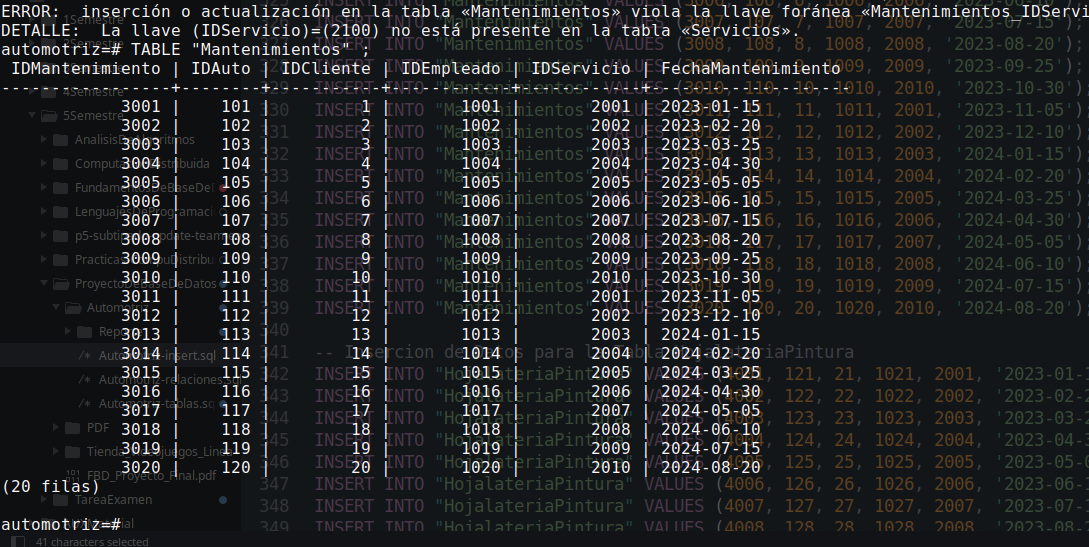
\includegraphics[width=1.0\textwidth]{H.png}
        \item Después de aplicar INSERT:
        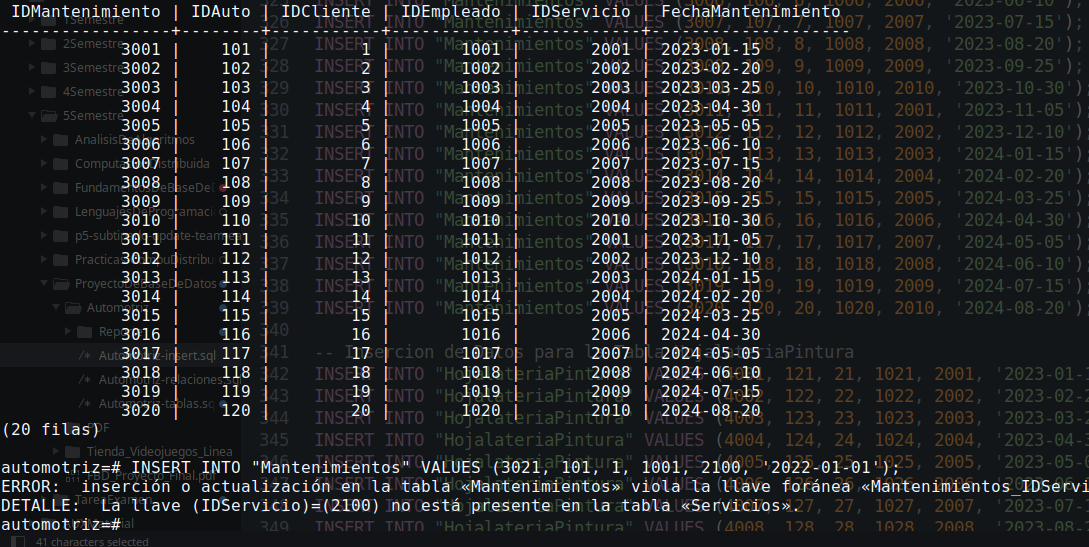
\includegraphics[width=1.0\textwidth]{I.png}
        \item[4.] Instrucción INSERT que cumple con las restricciones para tuplas:
        \begin{lstlisting}
INSERT INTO Mantenimientos ("IDAuto", "IDCliente", "IDEmpleado", "IDServicio", "FechaMantenimiento") VALUES (1, 1, 1, 101, '2023-01-01');
        \end{lstlisting}
        \item[5.] Captura de pantalla con el resultado de la instrucción que muestra que las restricciones para tuplas están funcionando:
        \item Antes de aplicar INSERT:
        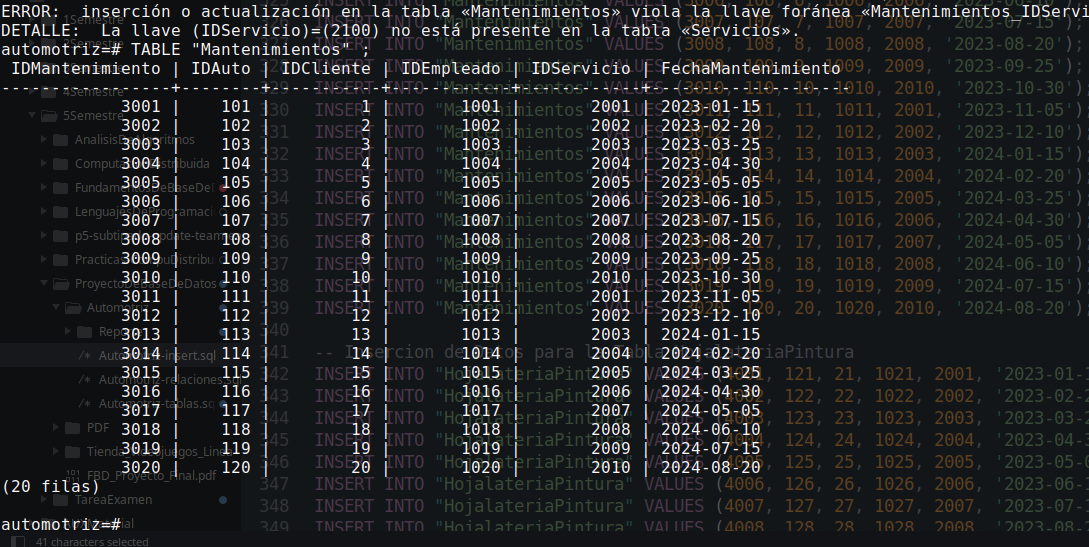
\includegraphics[width=1.0\textwidth]{H.png}
        \item Después de aplicar INSERT:
        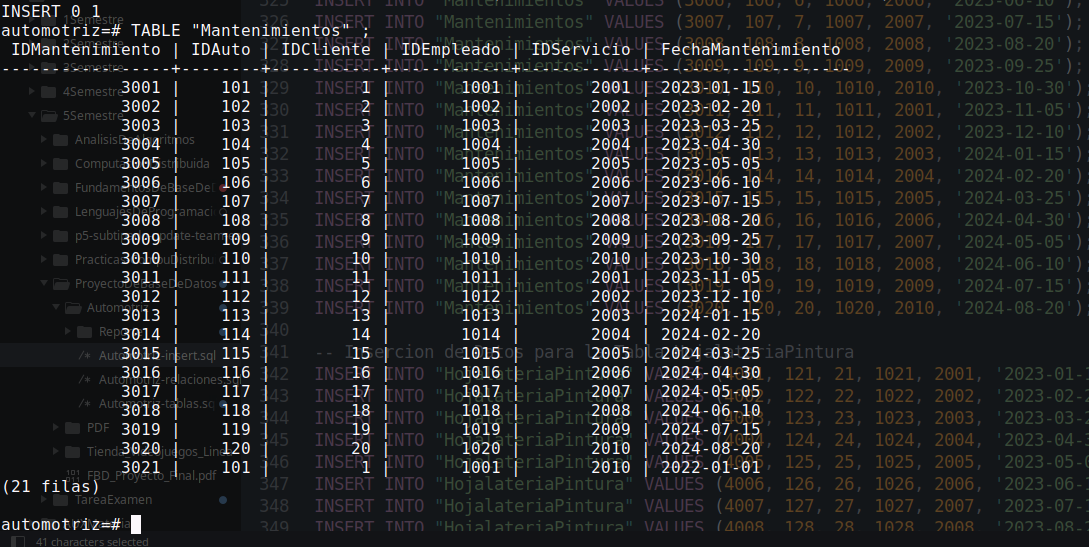
\includegraphics[width=1.0\textwidth]{J.png}
    \end{itemize}
    
    \subsection*{10. Consultas Relevantes}
    \begin{itemize}
        \item[a.1] Obtener la información de los clientes que han realizado mantenimientos a sus autos junto con los detalles de los mantenimientos.
        \item[b.1] Código en lenguaje SQL de la consulta:
        \begin{lstlisting}
SELECT
  c."IDCliente",
  c."Nombre" AS "NombreCliente",
  c."Direccion" AS "DireccionCliente",
  c."Telefono" AS "TelefonoCliente",
  m."IDMantenimiento",
  m."IDAuto",
  a."Marca",
  a."Modelo",
  m."FechaMantenimiento",
  s."NombreServicio",
  s."Descripcion",
  s."Precio" AS "PrecioServicio"
FROM
  "Clientes" c
JOIN
  "Mantenimientos" m ON c."IDCliente" = m."IDCliente"
JOIN
  "Autos" a ON m."IDAuto" = a."IDAuto"
JOIN
  "Servicios" s ON m."IDServicio" = s."IDServicio";
    \end{lstlisting}
    \item[c.1] Capatura de la consulta
    \center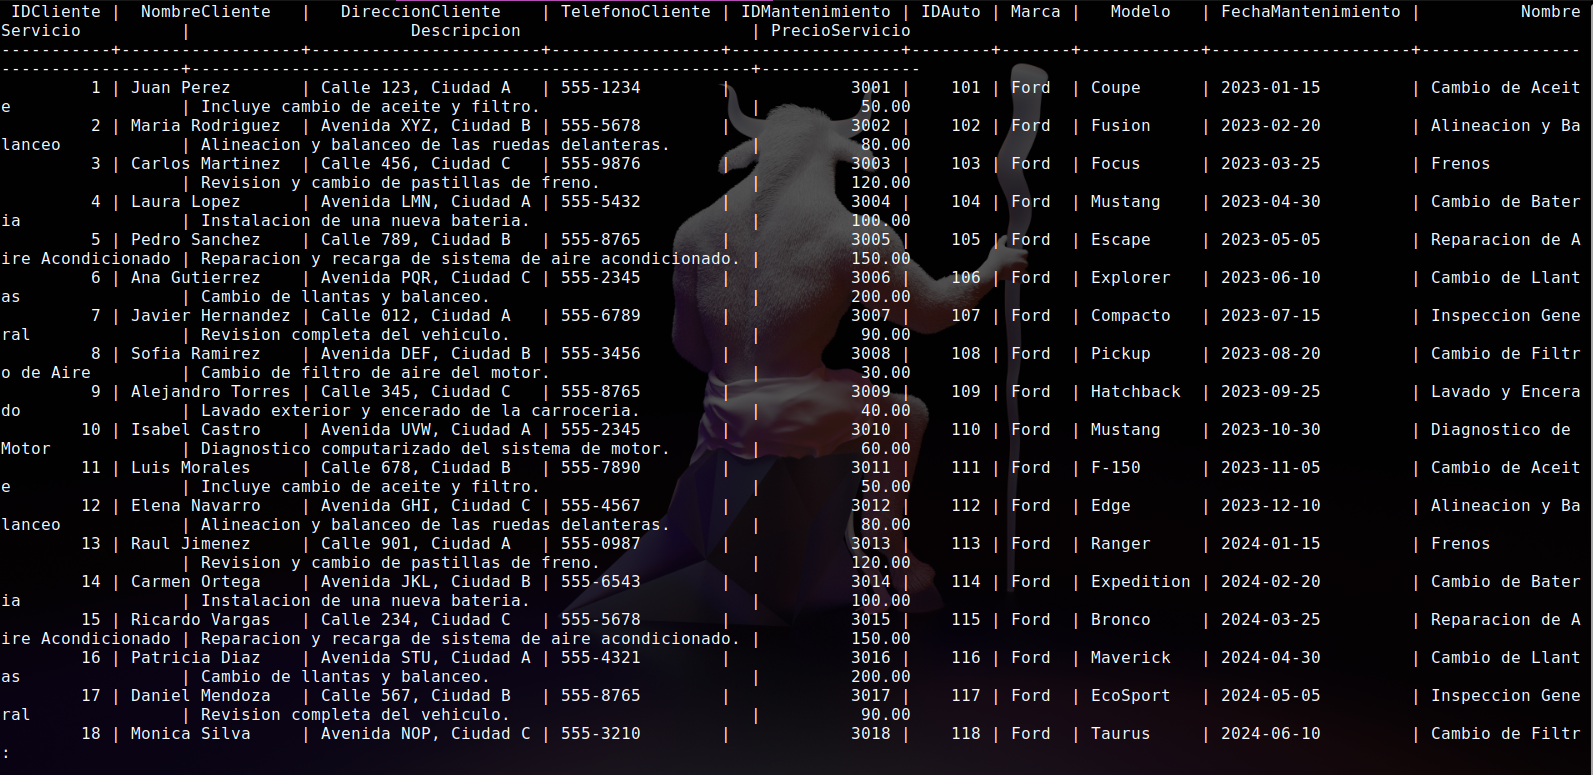
\includegraphics[width=1.0\textwidth]{K.png}
    \item[a.2] Obtener la cantidad total de autos que han sido sometidos a hojalatería y pintura, junto con su marca, agrupados por marca.
    \item[b.2] Código en lenguaje SQL de la consulta:
    \begin{lstlisting}
SELECT
  a."Marca",
  COUNT(hp."IDHojalateriaPintura") AS "CantidadAutosHojalateriaPintura"
FROM
  "Autos" a
LEFT JOIN
  "HojalateriaPintura" hp ON a."IDAuto" = hp."IDAuto"
GROUP BY
  a."Marca";
Consulta 3: Obtener la lista de empleados y la cantidad de mantenimientos que han realizado cada uno, ordenados de mayor a menor cantidad.
    \end{lstlisting}
    \item[c.2] Capatura de la consulta
    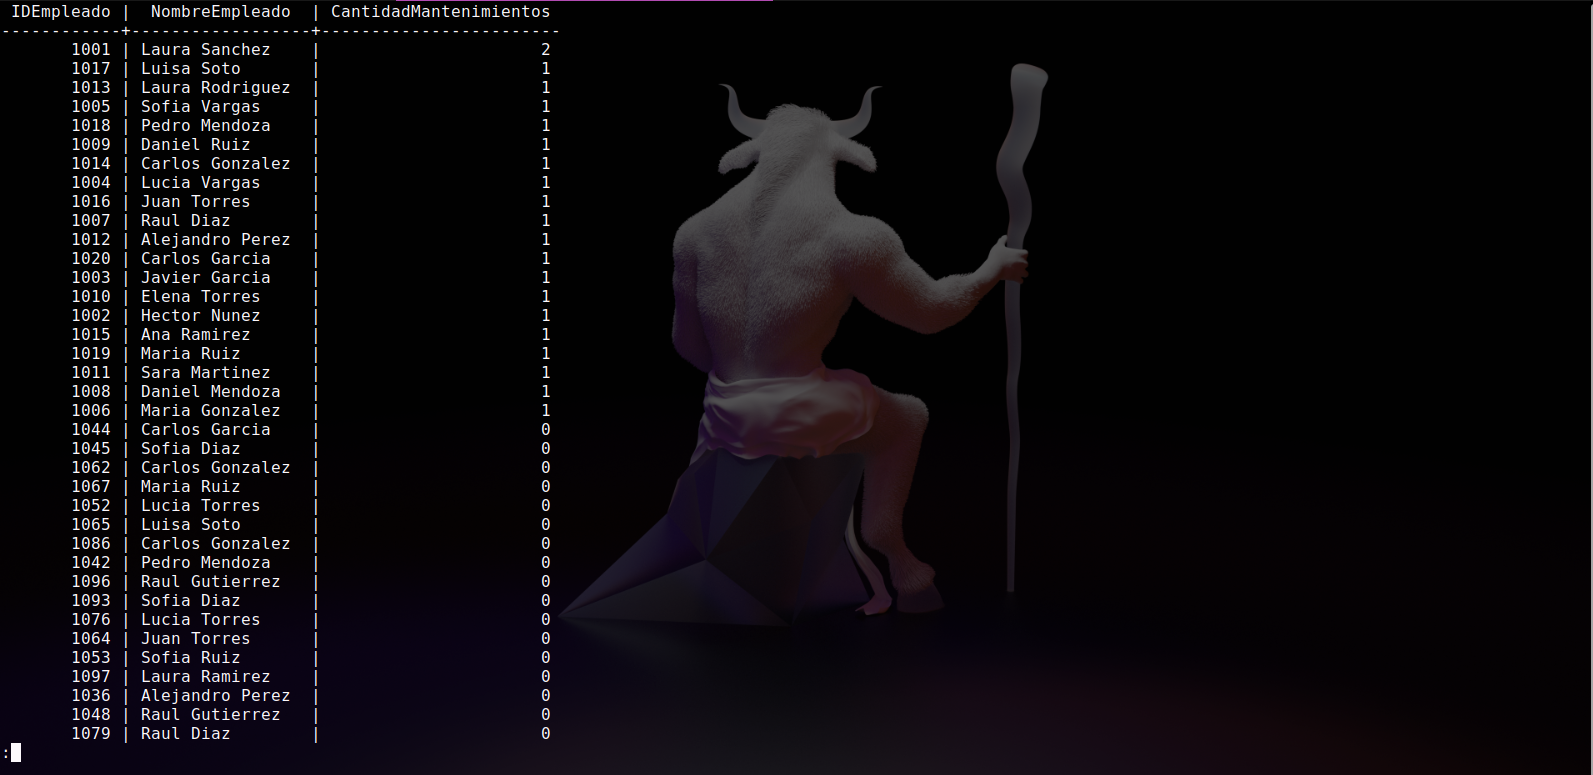
\includegraphics[width=1.0\textwidth]{L.png}
    \item[a.3] Obtener la lista de empleados y la cantidad de mantenimientos que han realizado cada uno, ordenados de mayor a menor cantidad.
    \item[b.3] Código en lenguaje SQL de la consulta:
    \begin{lstlisting}
SELECT
  e."IDEmpleado",
  e."Nombre" AS "NombreEmpleado",
  COUNT(m."IDMantenimiento") AS "CantidadMantenimientos"
FROM
  "Empleados" e
LEFT JOIN
  "Mantenimientos" m ON e."IDEmpleado" = m."IDEmpleado"
GROUP BY
  e."IDEmpleado", e."Nombre"
ORDER BY
  "CantidadMantenimientos" DESC;
    \end{lstlisting}
    \item[c.3] Capatura de la consulta
    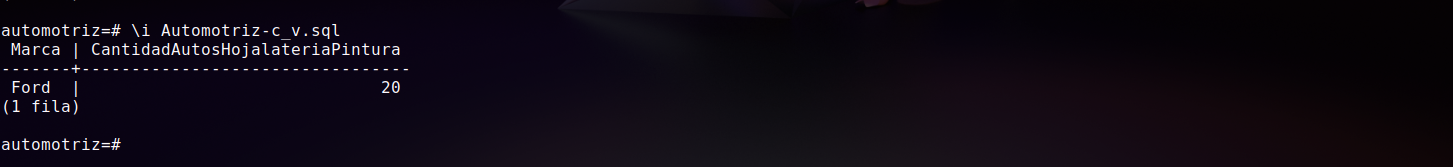
\includegraphics[width=1.0\textwidth]{M.png}
    \end{itemize}
    
    \subsection*{11. Vistas Relevantes}
    Vista 1: Información Detallada de Mantenimientos con Detalles de Clientes y Autos.
    \begin{itemize}
        \item[a] Vista que proporciona información detallada de los mantenimientos, incluyendo detalles de clientes y autos asociados.
        \item[b] Código en lenguaje SQL que permite crear la vista solicitada:
        \begin{lstlisting}
CREATE VIEW VistaMantenimientosDetallados AS
SELECT
  m."IDMantenimiento",
  c."IDCliente",
  c."Nombre" AS "NombreCliente",
  c."Direccion" AS "DireccionCliente",
  c."Telefono" AS "TelefonoCliente",
  a."IDAuto",
  a."Marca",
  a."Modelo",
  m."FechaMantenimiento"
FROM
  "Mantenimientos" m
JOIN
  "Clientes" c ON m."IDCliente" = c."IDCliente"
JOIN
  "Autos" a ON m."IDAuto" = a."IDAuto";
        \end{lstlisting}
        \item[c] Captura de la vista
        \center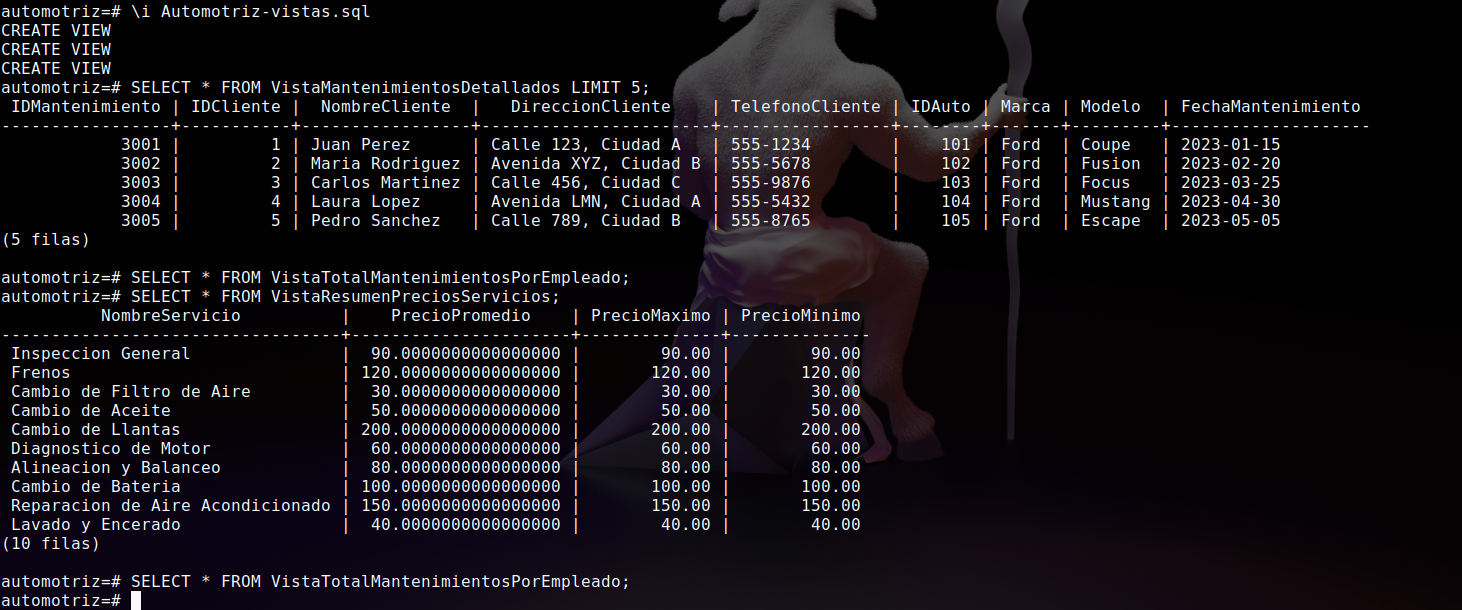
\includegraphics[width=1.0\textwidth]{N.png}
        \item[d] Ejemplo que los evaluadores pueden ejecutar para verificar el funcionamiento de la vista:
        \begin{lstlisting}
-- Seleccionar los primeros 5 registros de la vista
SELECT * FROM VistaMantenimientosDetallados LIMIT 5;
        \end{lstlisting}
    \end{itemize}
    Vista 2: Total de Mantenimientos Realizados por Cada Empleado.
    \begin{itemize}
        \item[a] Vista que muestra el total de mantenimientos realizados por cada empleado. 
        \item[b] Código en lenguaje SQL que permite crear la vista solicitada:
        \begin{lstlisting}
CREATE VIEW VistaTotalMantenimientosPorEmpleado AS
SELECT
  e."IDEmpleado",
  e."Nombre" AS "NombreEmpleado",
  COUNT(m."IDMantenimiento") AS "TotalMantenimientos"
FROM
  "Empleados" e
LEFT JOIN
  "Mantenimientos" m ON e."IDEmpleado" = m."IDEmpleado"
GROUP BY
  e."IDEmpleado", e."Nombre";
        \end{lstlisting}
        \item[c] Captura de la vista
        \center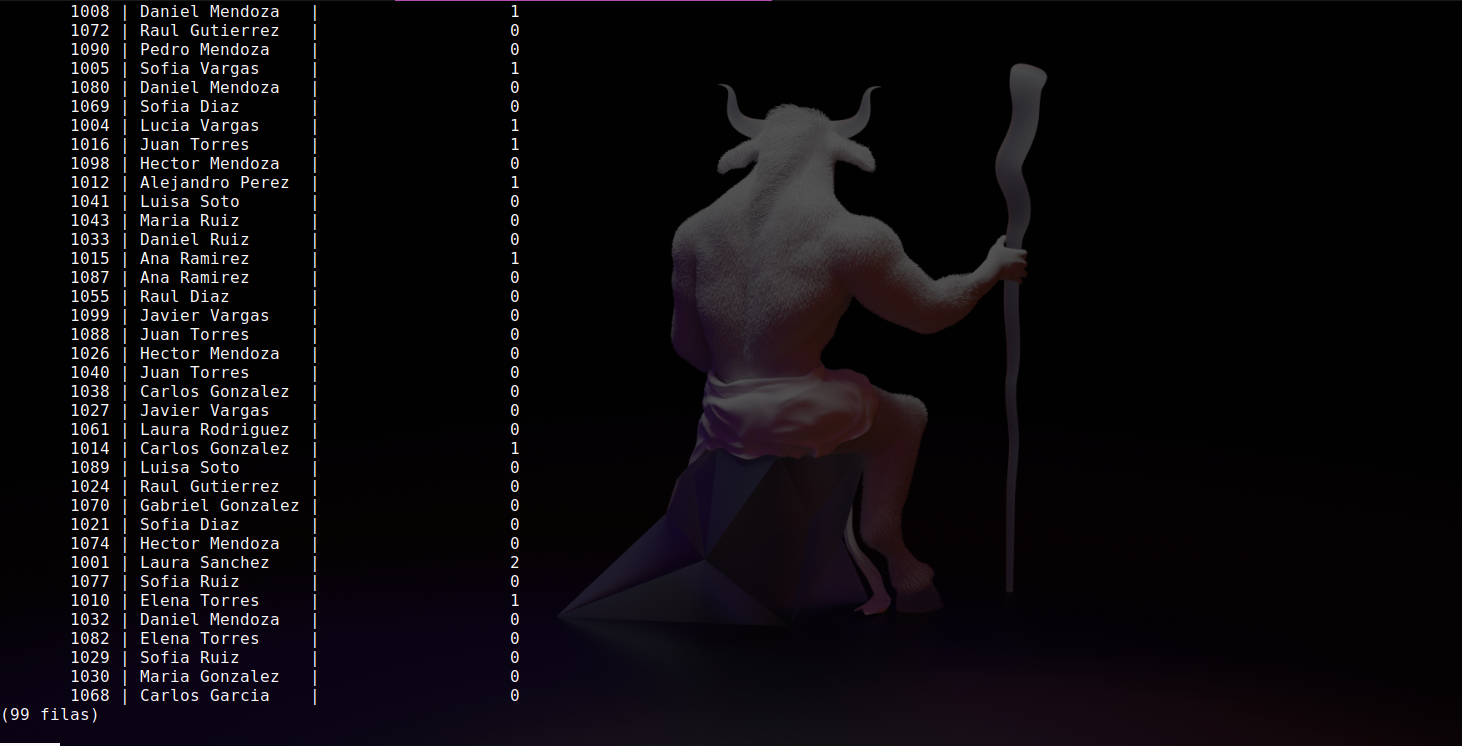
\includegraphics[width=1.0\textwidth]{O.png}
        \item[d] Ejemplo que los evaluadores pueden ejecutar para verificar el funcionamiento de la vista:
        \begin{lstlisting}
-- Seleccionar todos los registros de la vista
SELECT * FROM VistaTotalMantenimientosPorEmpleado;
         \end{lstlisting}
    \end{itemize}
    Vista 3: Resumen de Precios de Servicios Agrupados por Tipo de Servicio.
    \begin{itemize}
        \item[a] Vista que proporciona un resumen de los precios de los servicios agrupados por tipo de servicio.
        \item[b] Código en lenguaje SQL que permite crear la vista solicitada:
        \begin{lstlisting}
CREATE VIEW VistaResumenPreciosServicios AS
SELECT
  "NombreServicio",
  AVG("Precio") AS "PrecioPromedio",
  MAX("Precio") AS "PrecioMaximo",
  MIN("Precio") AS "PrecioMinimo"
FROM
  "Servicios"
GROUP BY
  "NombreServicio";
        \end{lstlisting}
        \item[c] Captura de la vista
        \center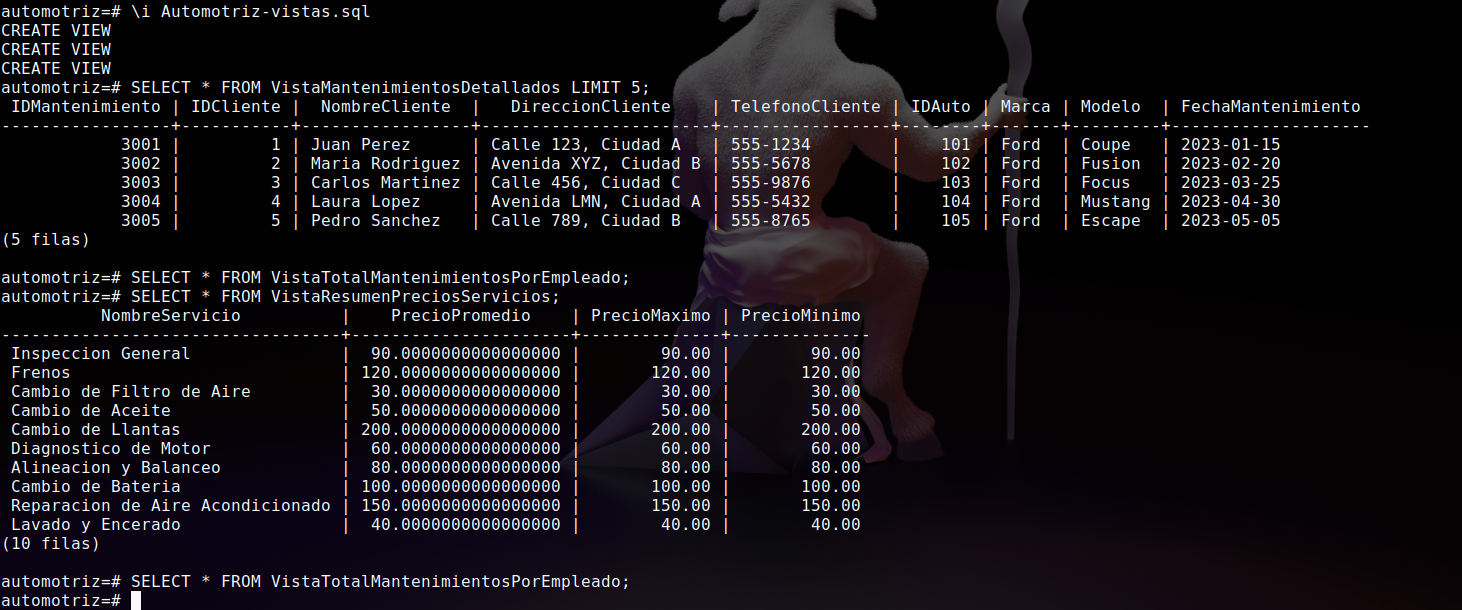
\includegraphics[width=1.0\textwidth]{N.png}
        \item[d] Ejemplo que los evaluadores pueden ejecutar para verificar el funcionamiento de la vista:
        \begin{lstlisting}
-- Seleccionar todos los registros de la vista
SELECT * FROM VistaResumenPreciosServicios;
        \end{lstlisting}
    \end{itemize}
\end{document}

